\renewcommand*{\arraystretch}{1.1}

\subsection*{BI / read / 14}
\label{section:bi-read-14}

% change \emph{} to use sans-serif font
\let\oldemph\emph
\renewcommand{\emph}[1]{{\footnotesize \sf #1}}

\renewcommand{\currentQueryCard}{14}
\marginpar{
	\raggedleft
	\vspace{0.22ex}

	\queryRefCard{bi-read-01}{BI}{1}\\
	\queryRefCard{bi-read-02}{BI}{2}\\
	\queryRefCard{bi-read-03}{BI}{3}\\
	\queryRefCard{bi-read-04}{BI}{4}\\
	\queryRefCard{bi-read-05}{BI}{5}\\
	\queryRefCard{bi-read-06}{BI}{6}\\
	\queryRefCard{bi-read-07}{BI}{7}\\
	\queryRefCard{bi-read-08}{BI}{8}\\
	\queryRefCard{bi-read-09}{BI}{9}\\
	\queryRefCard{bi-read-10}{BI}{10}\\
	\queryRefCard{bi-read-11}{BI}{11}\\
	\queryRefCard{bi-read-12}{BI}{12}\\
	\queryRefCard{bi-read-13}{BI}{13}\\
	\queryRefCard{bi-read-14}{BI}{14}\\
	\queryRefCard{bi-read-15}{BI}{15}\\
	\queryRefCard{bi-read-16}{BI}{16}\\
	\queryRefCard{bi-read-17}{BI}{17}\\
	\queryRefCard{bi-read-18}{BI}{18}\\
	\queryRefCard{bi-read-19}{BI}{19}\\
	\queryRefCard{bi-read-20}{BI}{20}\\
	\queryRefCard{bi-read-21}{BI}{21}\\
	\queryRefCard{bi-read-22}{BI}{22}\\
	\queryRefCard{bi-read-23}{BI}{23}\\
	\queryRefCard{bi-read-24}{BI}{24}\\
	\queryRefCard{bi-read-25}{BI}{25}\\
}



\noindent\begin{tabularx}{\queryCardWidth}{|>{\queryPropertyCell}p{\queryPropertyCellWidth}|X|}
	\hline
	query & BI / read / 14 \\ \hline
%
	title & Top thread initiators \\ \hline
%
	pattern & \multicolumn{1}{c|}{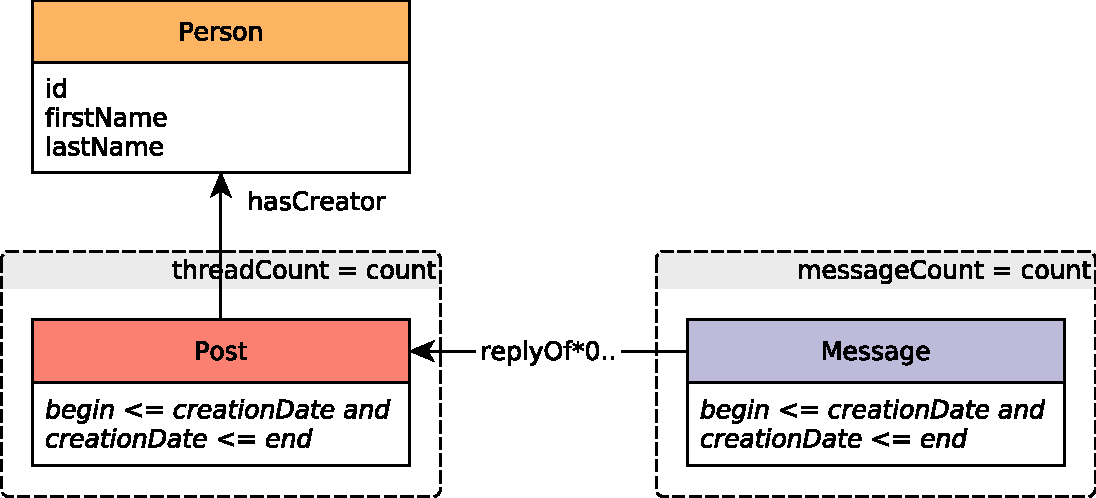
\includegraphics[scale=\patternscale,margin=0cm .2cm]{patterns/bi-read-14}} \\ \hline
%
	desc. & For each \emph{Person}, count the number of \emph{Posts} they created in
the time interval \texttt{{[}startDate,\ endDate{]}} (equivalent to the
number of threads they initiated) and the number of \emph{Messages} in
each of their (transitive) reply trees, including the root \emph{Post}
of each tree. When calculating \emph{Message} counts only consider
messages created within the given time interval.

Return each \emph{Person}, number of \emph{Posts} they created, and the
count of all \emph{Messages} that appeared in the reply trees (including
the \emph{Post} at the root of tree) they created.
 \\ \hline
%
	
		params &
		\innerCardVSpace{\begin{tabularx}{\attributeCardWidth}{|>{\paramNumberCell}c|>{\varNameCell}M|>{\typeCell}m{\typeWidth}|Y|} \hline
		$\mathsf{1}$ & startDate
 & Date
 &  \\ \hline
		$\mathsf{2}$ & endDate
 & Date
 &  \\ \hline
		\end{tabularx}}\innerCardVSpace \\ \hline
	
%
	
		result &
		\innerCardVSpace{\begin{tabularx}{\attributeCardWidth}{|>{\resultNumberCell}c|>{\varNameCell}M|>{\typeCell}m{\typeWidth}|>{\resultOriginCell}c|Y|} \hline
		$\mathsf{1}$ & person.id & 64-bit Integer & R &
				 \\ \hline
		$\mathsf{2}$ & person.firstName & String & R &
				 \\ \hline
		$\mathsf{3}$ & person.lastName & String & R &
				 \\ \hline
		$\mathsf{4}$ & threadCount & 32-bit Integer & A &
				The number of \emph{Posts} created by that \emph{Person} (the number of
threads initiated)
 \\ \hline
		$\mathsf{5}$ & messageCount & 32-bit Integer & A &
				The number of \emph{Messages} created in all the threads this
\emph{Person} initiated
 \\ \hline
		\end{tabularx}}\innerCardVSpace \\ \hline
	
%
	
		sort		&
		\innerCardVSpace{\begin{tabularx}{\attributeCardWidth}{|>{\sortNumberCell}c|>{\varNameCell}M|>{\directionCell}c|Y|} \hline
		$\mathsf{1}$ & messageCount
 & $\desc
$ &  \\ \hline
		$\mathsf{2}$ & person.id
 & $\asc
$ &  \\ \hline
		\end{tabularx}}\innerCardVSpace \\ \hline
	%
	limit & 100 \\ \hline
	%
	CPs &
	\multicolumn{1}{>{\raggedright}l|}{
		\chokePoint{1.2}, 
		\chokePoint{2.2}, 
		\chokePoint{2.3}, 
		\chokePoint{3.2}, 
		\chokePoint{7.2}, 
		\chokePoint{7.3}, 
		\chokePoint{7.4}, 
		\chokePoint{8.1}, 
		\chokePoint{8.5}
		} \\ \hline
	%
	%
\end{tabularx}
\queryCardVSpace

% change \emph back to the old one
\let\emph\oldemph